\documentclass[border=10pt]{standalone}
\usepackage{tikz}
\usetikzlibrary{shapes, arrows.meta, positioning, shadows, decorations.pathmorphing, calc}

\begin{document}

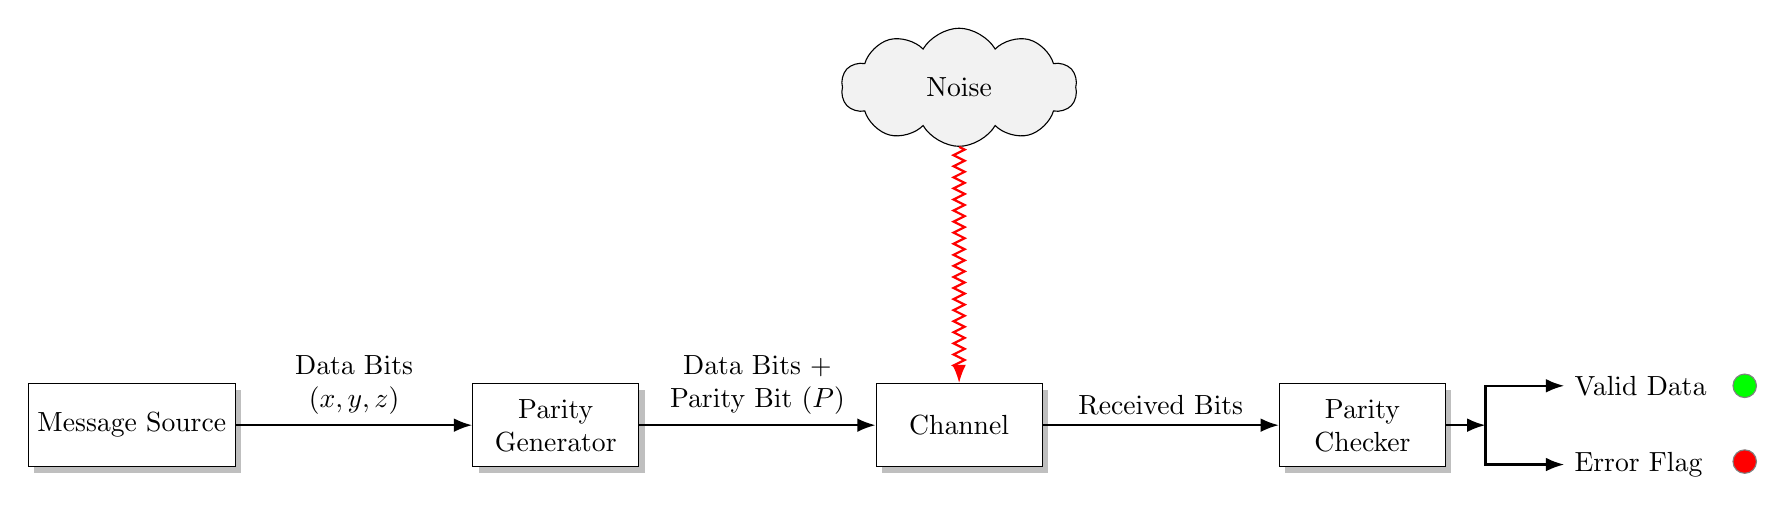
\begin{tikzpicture}[
    auto,
    node distance = 3cm,
    block/.style = {draw, rectangle, minimum height=3em, minimum width=6em, align=center, fill=white, drop shadow},
    sum/.style = {draw, circle, node distance=1cm},
    input/.style = {coordinate},
    output/.style = {coordinate},
    line/.style = {-Latex, thick},
    jagged/.style = {decorate, decoration={zigzag, segment length=4pt, amplitude=2pt, post=lineto, post length=5pt}}
]

    % Nodes
    \node [block] (source) {Message Source};
    \node [block, right=of source] (encoder) {Parity\\Generator};
    \node [block, right=of encoder] (channel) {Channel};
    \node [block, right=of channel] (decoder) {Parity\\Checker};
    \node [coordinate, right=of decoder] (sink) {};

    % Noise
    \node [cloud, draw, cloud puffs=10, cloud puff arc=120, aspect=2, inner sep=0, above=of channel, fill=gray!10, minimum width=3cm, minimum height=1.5cm] (noise) {Noise};

    % Edges
    \draw [line] (source) -- node [midway, align=center] {Data Bits\\($x,y,z$)} (encoder);
    \draw [line] (encoder) -- node [midway, align=center] {Data Bits +\\Parity Bit ($P$)} (channel);
    \draw [line] (channel) -- node [midway, align=center] {Received Bits} (decoder);
    
    % Noise Interference
    \draw [-Latex, thick, jagged, red] (noise) -- (channel.north);

    % Output edges from decoder
    \draw [line] (decoder.east) -- ++(0.5,0) coordinate (split);
    \draw [line] (split) |- ++(1,0.5) node [right] (vdata) {Valid Data};
    \node [circle, fill=green, draw=black!50, inner sep=3pt, right=0.2cm of vdata] (green_dot) {};
    \draw [line] (split) |- ++(1,-0.5) node [right] (err) {Error Flag};
    \node [circle, fill=red, draw=black!50, inner sep=3pt, below=0.65cm of green_dot] (red_dot) {};

\end{tikzpicture}

\end{document}
